\chapter{Facial Recognition}\label{ch:face-rec}
Facial recognition is a task of verifying or identifying a person from digital image/video.

As I mentioned in the definition, there are two main subtasks~\cite{FaceRec}:
\begin{enumerate}
    \item \textbf{Verification} deals with verifying whether the person in the image is who he claims he is.
    Typical modern use case of verification is smartphone unlocking with face.
    An example of such system is Face ID developed by Apple Inc.

    \item \textbf{Identification} is a task of matching a person to an identity.
    To formulate it in another way, the goal of identification is to give us an answer to the question of who the person
    in the image is.
\end{enumerate}

\section{Pipeline}\label{sec:pipeline}

Facial recognition pipeline\footnote{A chain of processing elements, arranged so that the output of each element is the
input of the next.} usually has the following four steps:
\begin{enumerate}
    \item The first on is \textbf{face detection} and it deals with determination of face location within the image.
    The output of the algorithm is usually face coordinates and facial landmarks.
    Landmarks are a set of coordinates marking important points of the face (eyebrows, nose, mouth, \ldots).
    The knowledge of these points is a necessity for the following step.
    \item \textbf{Face alignment} is a task of changing the face position in such a way that it resembles the position
    of faces on which the feature extraction model was trained.
    In most of the instances this step improves the accuracy.
    \item \textbf{Feature extraction} is a process of computing a feature vector\footnote{A feature vector is a vector
    that contains information describing an object's important characteristics.} of the face.
    Architecture of models used for feature extraction is described in section~\ref{sec:mod-methods}.
    \item \textbf{Feature matching} uses feature vector from the previous task to identify the person in the image.
    The algorithm uses a database of pre-computed feature vectors and compares them to the newly extracted one.
    The identity associated with the feature vector which has the smallest distance from the extracted one is
    considered to be the identity of the person in the image.
\end{enumerate}

\section{Overview of Modern Methods}\label{sec:mod-methods}
In this section I am about to provide an overview of modern methods/models used for facial recognition.
Models based on CNN architecture~\ref{ch:cnn} achieve state-of-the-art results which is the reason why CNNs dominate the
field of facial recognition and the field of computer vision as a whole now.

Innovations made in the field of computer vision are usually applicable to the subfield of facial recognition as well.
This is manifested in usage of the same model architectures in general image classification as well as in facial
recognition.
However there is a lot of innovation going on in the design of loss functions which work specifically well when used for
model training\footnote{Machine learning task of learning a function that maps an input to an output based on example
input-output pairs.} in facial recognition tasks.
This is the reason why this section is divided in two parts: \textit{models}~\ref{subsec:models} and
\textit{loss functions}~\ref{subsec:loss-functions}.

\subsection{Models}\label{subsec:models}

\subsubsection{DeepFace}\label{subsubsec:deepface}
DeepFace~\cite{DeepFace} is a system developed by FaceBook Inc. in 2014.

The research is notable for its use of advanced alignment technique which consists of three steps:

\begin{enumerate}
    \item The first step is \textbf{2D Alignment} and it begins with detection of 6 fiducial points/landmarks.
    These points and the reference position of points are then used to find a transformation.
    This transformation then generates 2D aligned and cropped image.
    \item The second step is \textbf{3D Alignment}.
    In this step the image is warped onto a generic 3D shape model.
    This is achieved by localization of 67 fiducial points in the image and then fitting an affine
    camera\footnote{linear mathematical model to approximate the perspective projection followed by an ideal
    pinhole camera.} \textit{P} using the generalized least squares solution and the reference position $x_{3d}$ of
    points on the 3D shape model.
    \item \textbf{Frontalization} is the final step and it is achieved by a piece-wise affine transformation T from
    $x_{2d}$ source to $\tilde{x_{3d}}$ target.
    The target $\tilde{x_{3d}}$ is a list of positions of reference fiducial points from previous step enriched with
    residuals \textit{r}.
    These residuals were added to the reference positions $\tilde{x_{3d}}$ to account for non-rigid deformations which
    are not modeled by the affine camera \textit{P}.
    Without these residuals, all faces would be warped into the same shape losing important discriminative factors.
\end{enumerate}

\begin{figure}[H]
    \centering
    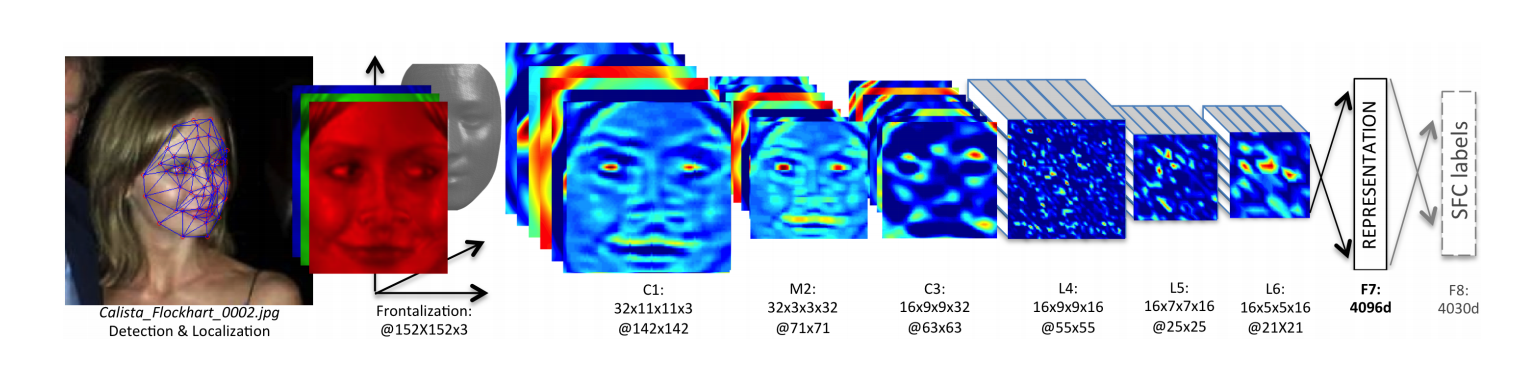
\includegraphics[width=\columnwidth]{images/face-recognition/deepface.png}
    \caption{Outline of DeepFace architecture~\cite{DeepFace}}
    \label{fig:deepface}
\end{figure}

There are 9 layers in the model with over 120 million parameters.
The process of classification is visualized in the picture~\ref{fig:deepface}.
The model was trained on more than 4 million images and as the name of the research paper~\cite{DeepFace} implies, the
results (\textbf{97.35\%} on LFW dataset) almost matched the results of humans (\textbf{97.53\%} on LFW dataset).


\subsubsection{FaceNet}\label{subsubsec:facenet}
FaceNet~\cite{FaceNet} is a system developed by researchers from Google Inc. in 2015.

Interesting innovation of FaceNet lies in the format of its output.
The output of the network is a vector representing a position in an euclidean space (so called embeddings) instead of a
number representing identity.
This approach allows for straight-forward implementation of \textit{verification} and
\textit{identification}~\ref{ch:face-rec}.
Implementation of verification involves thresholding the distance between two embeddings; and identification becomes
k-NN classification problem.

\begin{figure}[H]
    \centering
    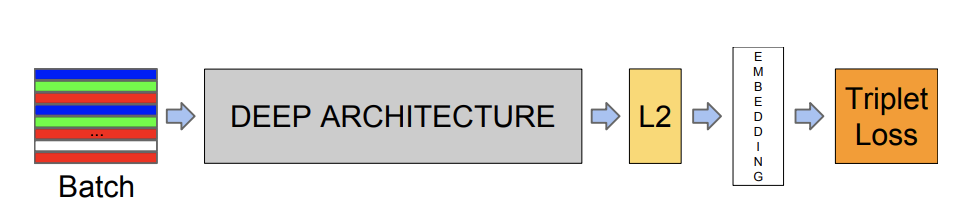
\includegraphics[width=\columnwidth]{images/face-recognition/facenet.png}
    \caption{Outline of FaceNet architecture~\cite{FaceNet}}
    \label{fig:facenet}
\end{figure}

The architecture of the model is based on CNNs~\ref{ch:cnn} and loss function used to train the model is called
\textit{triplet loss}~\ref{subsubsec:triplet-loss}.

The advantages of the model are its accuracy and the compactness of the face representation.
The accuracy of the model exceeded that of human with \textbf{99.63\%} on LFW dataset and the euclidean space has only
128 dimensions.
Another advantage is that the model achieved great results on faces which are not in ideal position without using any
of the complex 3D modeling techniques (as was the case in DeepFace system~\ref{subsubsec:deepface}).
To use proper terms the system is \textit{pose invariant}.

\subsubsection{ResNet}\label{subsubsec:resnet}
A residual neural network (ResNet)~\cite{ResNet} is an ANN which allows for training of networks which contain tens
of layers.
Training of ANN this deep had been practically impossible before the invention of ResNet due to the problem of
\textit{vanishing gradient}\footnote{See footnote on page~\pageref{foot:vangrad}} and \textit{degradation problem}.
The first problem is exposed as a lack of convergence and the second one as a high training error.

Both of these problems have been avoided by implementation of \textit{skip connections} which are illustrated in
figure~\ref{fig:ResNet}.

\begin{figure}[H]
    \centering
    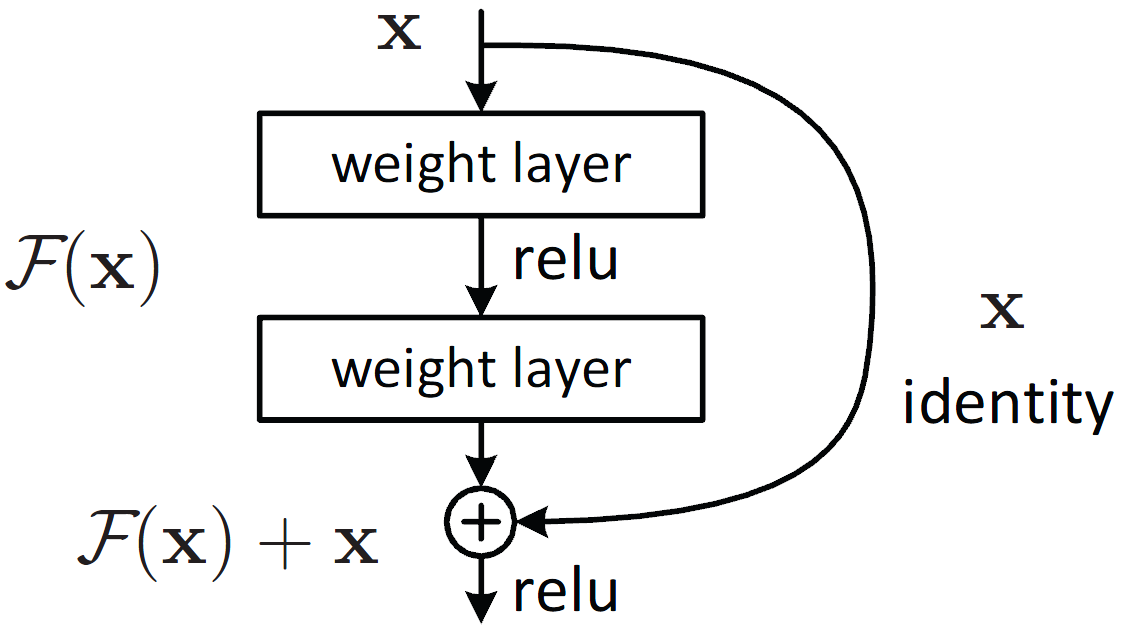
\includegraphics[width=0.9\columnwidth]{images/face-recognition/resnet.png}
    \caption{Residual learning~\cite{ResNet}}
    \label{fig:ResNet}
\end{figure}

The skip connections let the in-between layers fit a residual mapping.
This has proven to be an effective way of using deep neural networks to increase accuracy.

ResNets are widely used in the field of facial recognition as well as in the field of computer vision as a whole.

\subsubsection{InceptionNet}\label{subsubsec:inceptionnet}
InceptionNets are a class of models in which there are multiple kernel sizes operating at the same level.
This is desirable because the right kernel size is dependent on how globally the information is distributed.
A large kernel is preferred when the information is distributed globally and vice versa.

\begin{figure}[H]
    \centering
    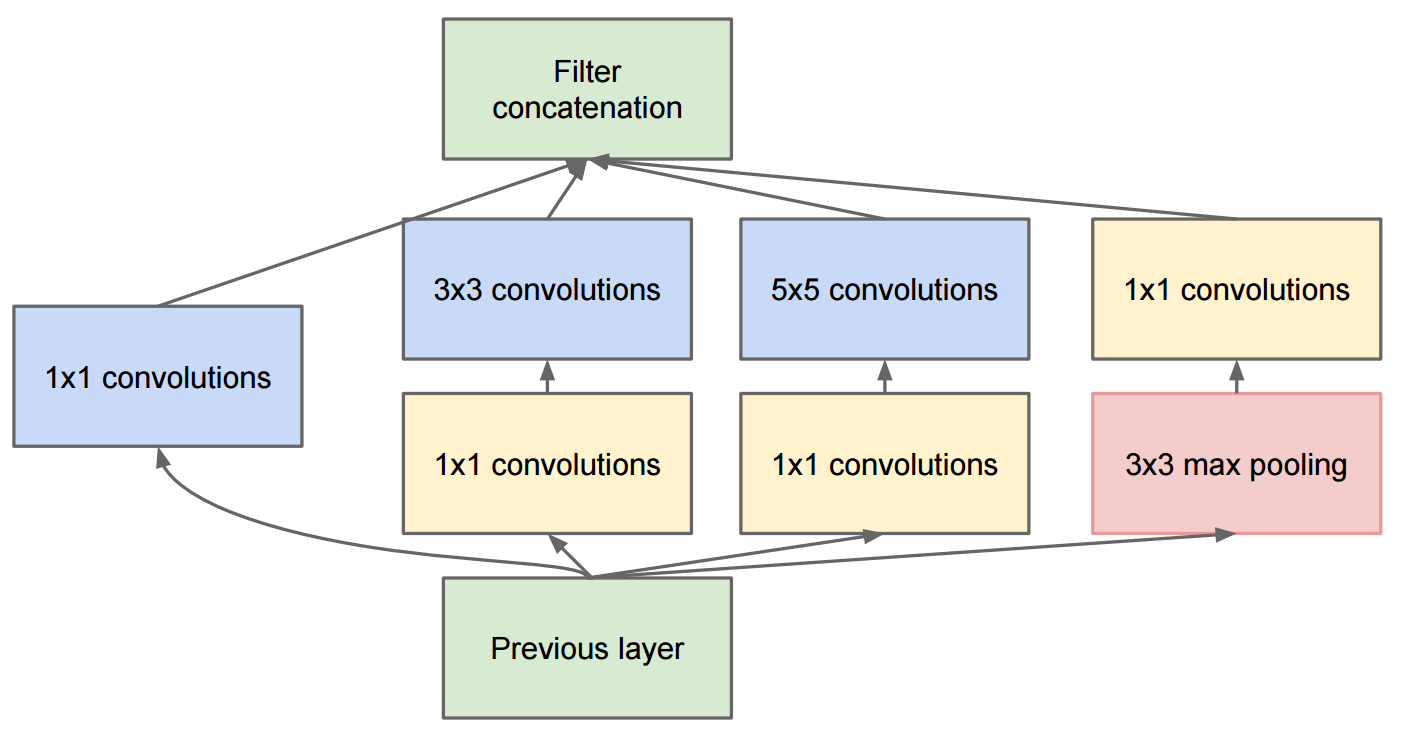
\includegraphics[width=0.9\columnwidth]{images/face-recognition/inceptionnet.png}
    \caption{InceptionNet block~\cite{GoingDeeper}}
    \label{fig:InceptionNet}
\end{figure}

The inception of the inception block (figure~~\ref{fig:InceptionNet}) took place in 2014 in the paper~\cite{GoingDeeper}
published by Google Inc.
Models using inception blocks kept on improving and at the time of writing there is fourth version in use.

\subsubsection{DenseNet}\label{subsubsec:densenet}
DenseNet~\cite{DenseNet} is a type of CNN~\ref{ch:cnn} which was introduced in 2017.
The difference from regular CNNs is that every layer is connected to all the subsequent layers.
Traditional CNN with \textit{L} layers has exactly \textit{L} connections.
On the other hand DenseNet with the same amount of layers contains $\frac{L\left( L+1 \right)}{2}$ connections.
The block of layers is illustrated in figure~\ref{fig:DenseNet}.

\begin{figure}[H]
    \centering
    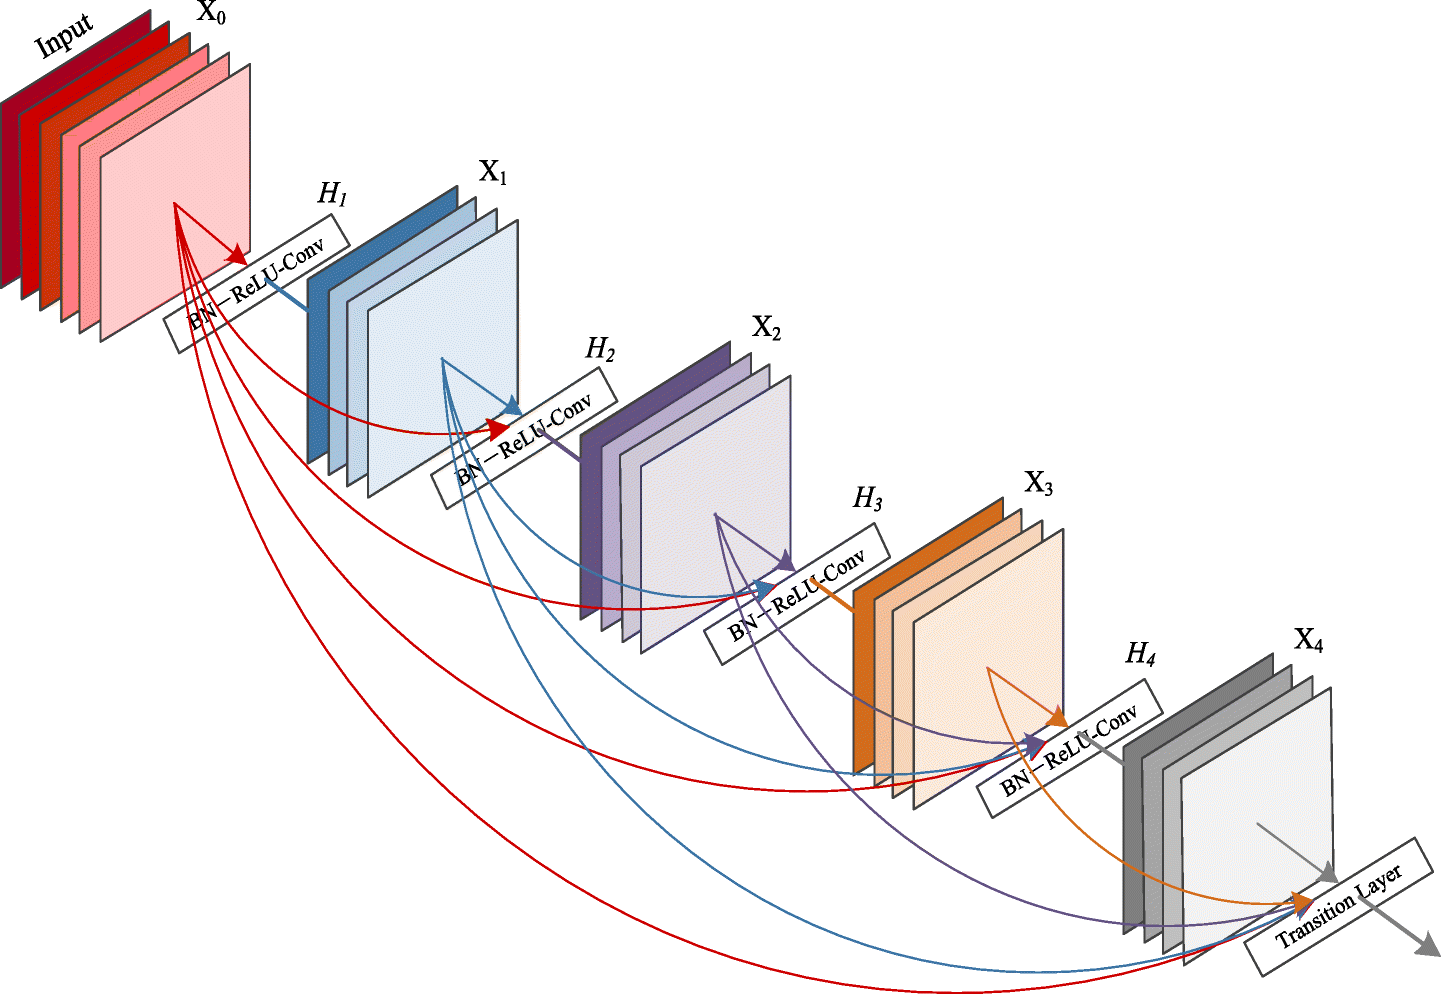
\includegraphics[width=0.9\columnwidth]{images/face-recognition/densenet.png}
    \caption{A 5-layer dense block~\cite{DenseNet}}
    \label{fig:DenseNet}
\end{figure}

DenseNets have several compelling advantages~\cite{DenseNet}.
They alleviate the vanishing-gradient problem, strengthen feature propagation, encourage feature reuse, and
substantially reduce the number of parameters.

\subsection{Loss Functions}\label{subsec:loss-functions}

\subsubsection{Triplet Loss}\label{subsubsec:triplet-loss}

\begin{figure}[H]
    \centering
    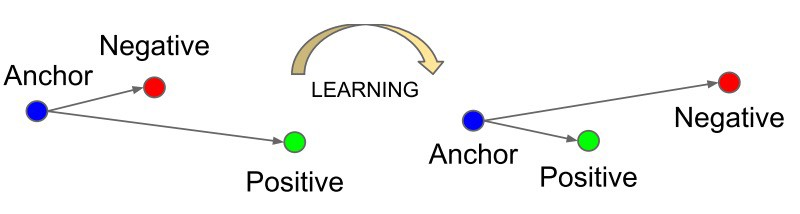
\includegraphics[width=\columnwidth]{images/face-recognition/tripletloss.jpeg}
    \caption{Illustration of the triplet loss~\cite{FaceNet}}
    \label{fig:tripletloss}
\end{figure}